\documentclass[../../submission.tex]{subfiles}
\begin{document}
\section{Result}

\subsection{Good ways to fix query (RSQ3)}
A significant challenge arises from the lack of transparency in artificial intelligence systems, 
particularly regarding the underlying processes and algorithms that generate results. 
Therefore, we surveyed the participants to ascertain how they would prefer to be assisted in the event that 
their preliminary search query did not align with their actual needs. The proponents advanced a number of 
intriguing concepts. For instance, the potential exists for the artificial intelligence to adjust the filters 
based on the user's search history. As illustrated in Figure \ref{fig:filter}, the potential appearance of the phenomenon is 
demonstrated. In this instance, the filter is dynamically adjusted. Therefore, the user is able to ascertain 
which filters the KI utilizes and, consequently, identify the potential origin of an error. Therefore, the user 
has the option of either utilizing the filter to resolve the issue or adjusting the initial search query.

\begin{figure}[h]
    \centering
    \begin{minipage}{0.35\textwidth}
        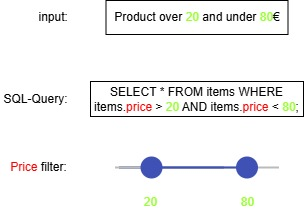
\includegraphics[width=\textwidth]{images/filter}
        \caption{AI dynamically adjusts the filters}
        \Description{}
        \label{fig:filter}
    \end{minipage}
    \hfill
    \begin{minipage}{0.55\textwidth}
        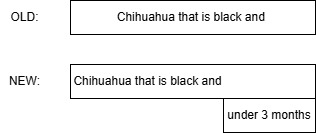
\includegraphics[width=\textwidth]{images/vorschlag}
        \caption{AI provides information on features that cannot be combined}
        \Description{}
        \label{fig:suggestions}
    \end{minipage}
\end{figure}
A further potential avenue for enhancing the efficacy of the user's 
outcomes is the implementation of an artificial intelligence system that can 
evaluate the combinability of diverse features during the user's input phase. 
In such a case, it is essential that the user be alerted to this possibility. 
As demonstrated in Figure \ref{fig:suggestions}, the initial state is displayed, denoting the current 
state of affairs.The subsequent version has been enhanced to alert the user to the 
absence of products for a given combination of features. In this instance, the 
"under 2 months" feature is distinctly emphasized, as it does not result in any products. 
Therefore, the user has the capacity to modify the preliminary search query and discern the 
elements that are not compatible. The integration of this concept with the search function 
can result in the automatic generation of suggestions for relevant features. This concept is 
further illustrated in Figure \ref{fig:suggestions}.

A further point to be considered is the potential for the AI to present analogous 
products in the event that the search yields minimal results. A relevant example  
would be a search for dogs that are of medium size. In the event that the available 
results are limited, the artificial intelligence could be programmed to display dogs of 
smaller stature.

\begin{figure}[h]
    \centering
    \begin{minipage}{0.45\textwidth}
        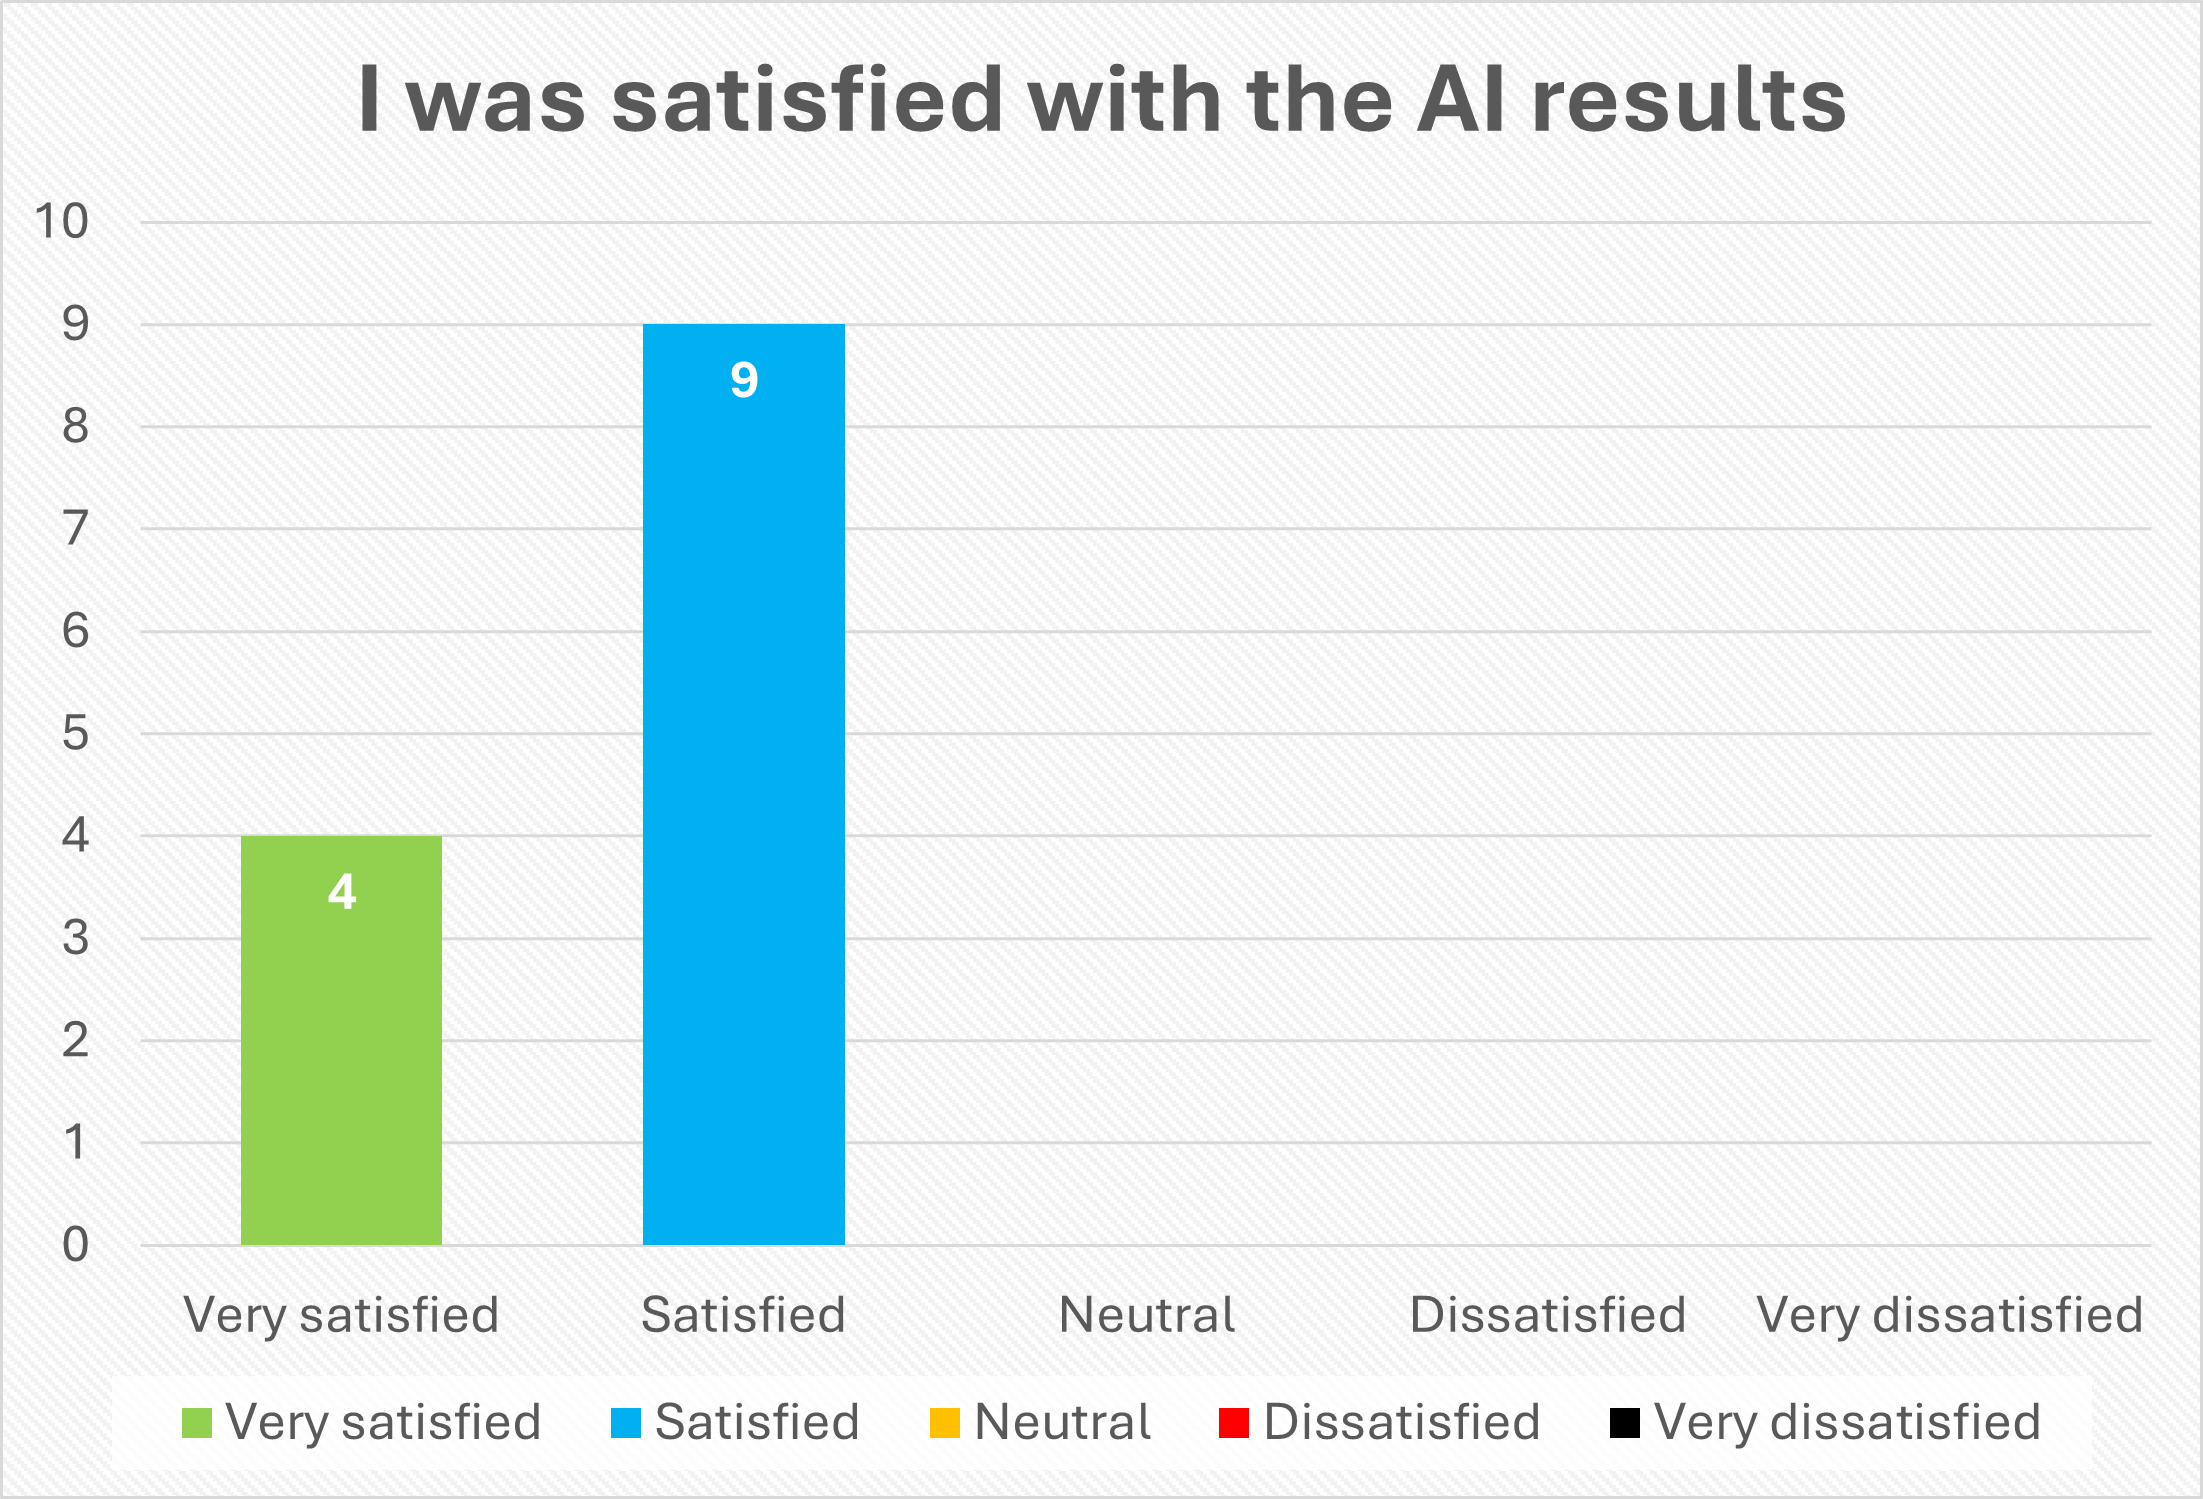
\includegraphics[width=\textwidth]{images/result_ki}
        \caption{AI dynamically adjusts the filters}
        \label{fig:result_KI}
    \end{minipage}
    \hfill
    \begin{minipage}{0.45\textwidth}
        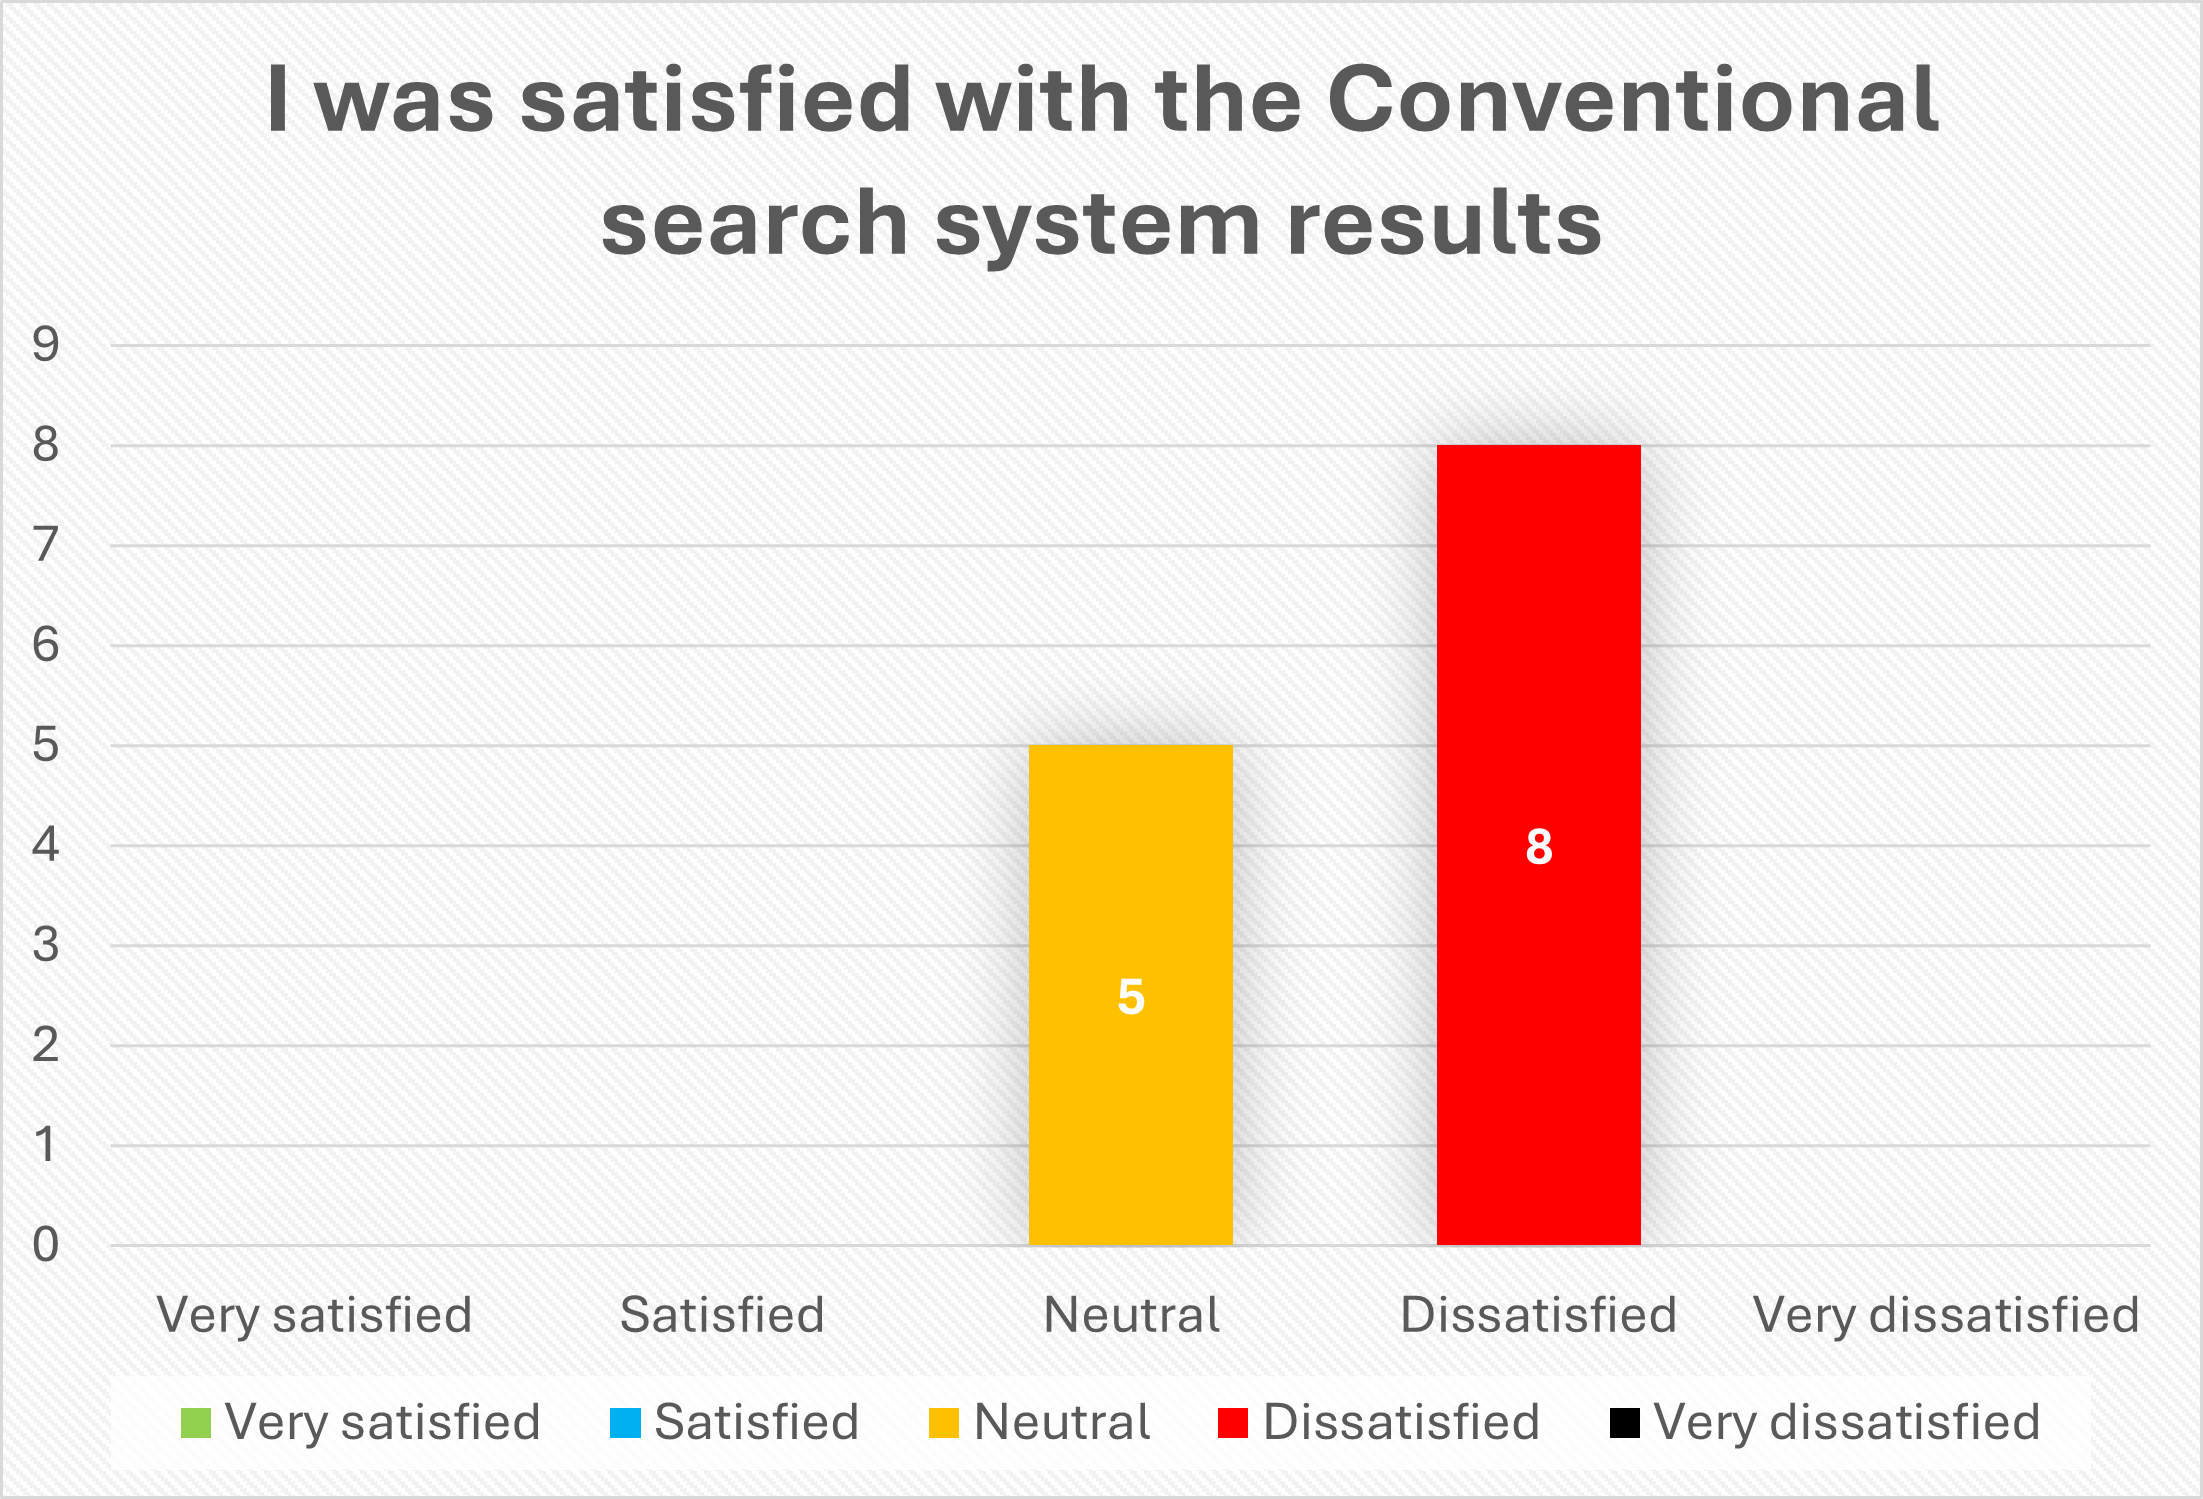
\includegraphics[width=\textwidth]{images/result_konv}
        \caption{AI provides information on features that cannot be combined}
        \Description{}
        \label{fig:result_Konv}
    \end{minipage}
\end{figure}


\subsection{User Satisfaction (RSQ5)}
A further aspect that was examined in our user study was the extent to which 
users expressed satisfaction with the outcomes produced by both the AI and 
conventional systems.

As illustrated in Figure \ref{fig:result_KI}, all participants who contributed to the study 
expressed satisfaction with the outcomes generated by the AI.  A considerable 
proportion of the users, amounting to 30\%, expressed profound satisfaction with 
the outcomes, attributing this positive sentiment to the effective comprehension 
of their intentions by the artificial intelligence system.

A review of the satisfaction levels observed in conventional systems clearly 
indicates a preference for AI, as demonstrated in Figure \ref{fig:result_Konv}. However, it should 
be noted that the study revealed a notable observation: the presence of a decline 
in the utilization of filters by users, coinciding with the enhanced comprehension 
of user intentions by the AI system. This phenomenon led to the suboptimal performance
 of the conventional system in comparison to the AI-based alternative. 
 Therefore, it is important to consider the potential for a filter bias. 
 Therefore, the users' discontent with the results is understandable. 
 It is possible that the results would have been more favorable had the experiment 
 been conducted differently.

 \subsection{Importance of Filters (RSQ7)}
 One of the objectives of the user study was to ascertain the 
 importance of filters for users in the context of search results. 
 This was particularly relevant in scenarios where the efficacy of search 
 engine algorithms in generating relevant results is already well-established. 

 \begin{figure}[h]
    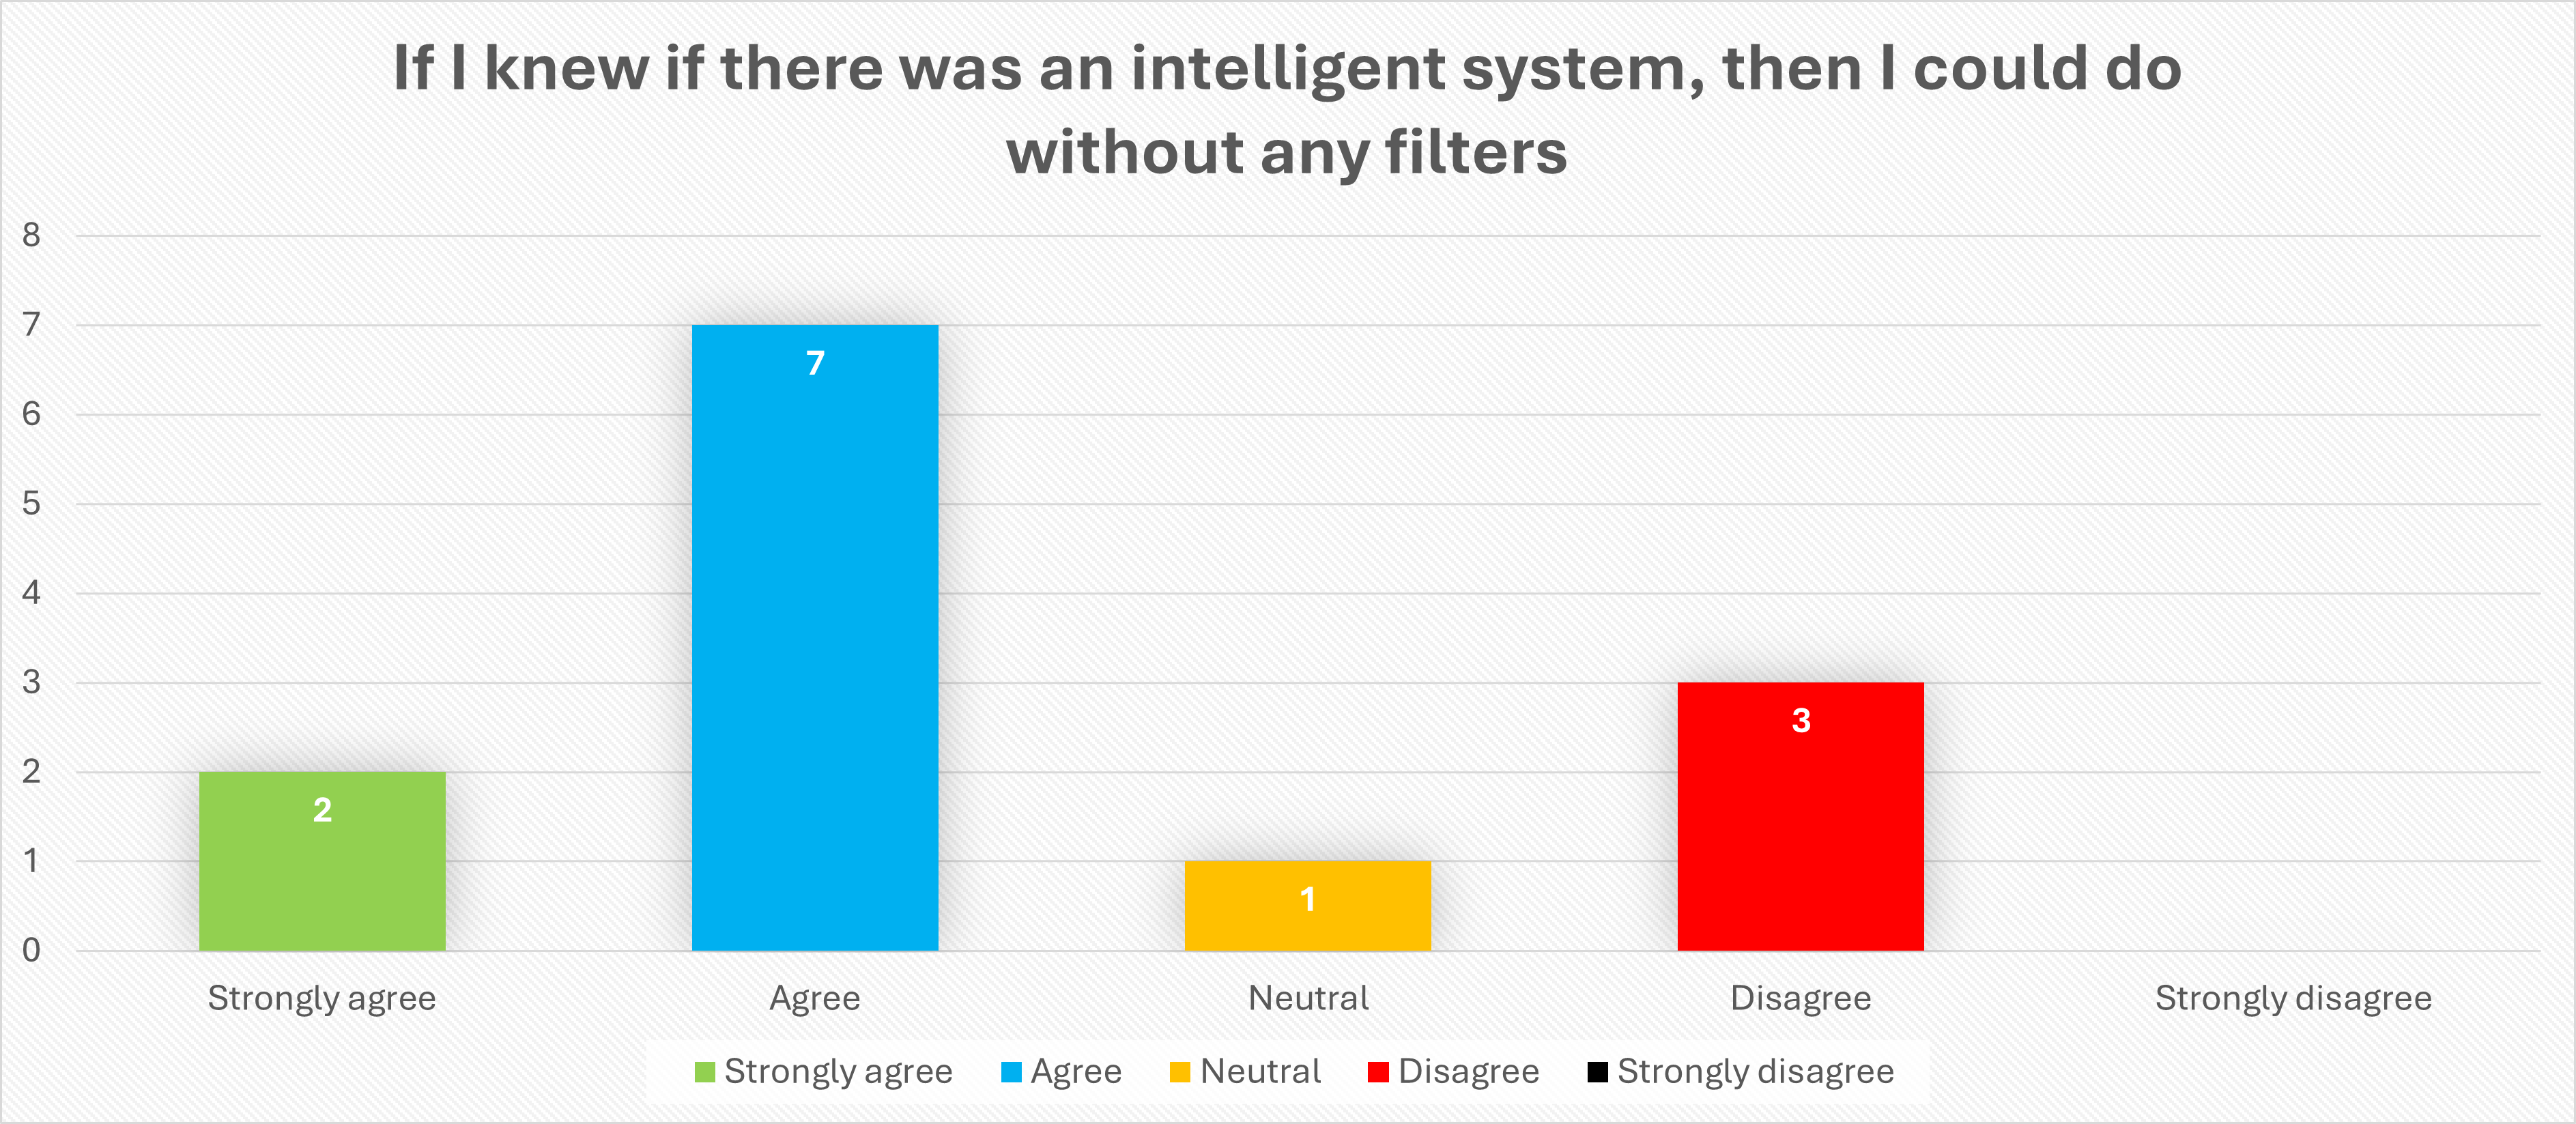
\includegraphics[width=\textwidth]{images/without_filter}
    \caption{AI provides information on features that cannot be combined}
    \Description{}
    \label{fig:without_filter}
 \end{figure}

 As illustrated in Figure \ref{fig:without_filter} , there is considerable variation in opinion among 
 the users. Approximately 70\% of users affirm that, should such a system be 
 in place, the absence of filters would be acceptable to them. Nonetheless, 
 approximately 20\% of respondents indicated a preference for maintaining web 
 filters, even in the context of a system that incorporates these filters. 
 The underlying reason for this phenomenon is that users prefer to utilize visual 
 filters, such as sorting or price filters, rather than using it through tipping. 
 The proponents indicated that the process of establishing the price filter is 
 straightforward. They noted that this is due to the ability to swiftly determine 
 the range of products in question, as opposed to the more cumbersome method of 
 manual calculation. Five of the propants who expressed agreement also indicated 
 a desire for additional practical filters, like the previously mentioned filters, 
 such as price and sorting. This additional desire for filters is the reason why 
 they did not strongly agree. Therefore, even if a system with AI is used, it is 
 important to maintain filters.

\end{document}